\documentclass[12pt]{article}

%%%%%%%%%%%%%%%%%%%%%%% Don't change anything in here. This space is called the preamble, it is where you tell the computer to load the proper LaTeX packages to perform the math and formatting desired. 
\usepackage{url}
\usepackage{multicol}
\usepackage{amsmath}
\usepackage{esint}
\usepackage{physics} 
\usepackage{siunitx}
\usepackage{bigints}
\usepackage{amsfonts}
\usepackage{textcomp}
\usepackage{xcolor}
\usepackage{tikz}
\usepackage{verbatim}
\usetikzlibrary{calc}
\usetikzlibrary{decorations.pathmorphing}
\usepackage{amsmath,amssymb}
\usepackage{siunitx} 
\usepackage{subcaption} 
\usepackage{blindtext} 
\usepackage{enumerate} 
\usepackage{pgfplots}
\usepackage{graphicx}
\usepackage{dsfont}
\usepackage{float}
\bibliographystyle{iopart-num}
\usepackage{cite}
\usepackage{wrapfig} %preámbulo
\usepackage{enumitem}
\usepackage{pgfplotstable}
\usepackage[compact]{titlesec}  
\usepackage[document]{ragged2e}
\usepackage{tikz,pgfplots}
\usepackage[spanish]{babel}
\usepackage[utf8]{inputenc}
\usepackage{hyperref}
\usepackage{amsmath, amsthm, amssymb}  %I added this so that you can use the align tool for equations!
\usepackage{colortbl}
\usepackage{mathtools}
\usepackage{sectsty}
\usepackage{esint}
\usepackage[makeroom]{cancel}
\usepackage{pgfplots}
\usepackage{graphicx}
\usepackage{dsfont}
\usepackage{float}
\usepackage{pdfpages}
\bibliographystyle{iopart-num}
\usepackage{cite}
\usepackage{wrapfig} %preámbulo
\usepackage{enumitem}
\usepackage{pgfplotstable}
\usepackage[compact]{titlesec}  
\usepackage[document]{ragged2e}
\usepackage{tikz,pgfplots}
\usepackage[spanish]{babel}
\usepackage[utf8]{inputenc}
\usepackage{hyperref}
\newtheorem{thm}{Teorema}[subsection]
\newtheorem{teo}[thm]{Teorema}
\newtheorem{obss}{Obs}[subsection]
\newtheorem{defff}{Def}[subsection]
\newtheorem{conjeture}{Conj}[subsection]
\newtheorem{defn}[defff]{Definición}
\newtheorem{lem}{Lemma}[thm]
\newtheorem{cor}{Corollary}[thm]
\newtheorem{prop}{Proposition}[thm]
\newtheorem{rem}{Remark}[thm]
\newtheorem{ill}{Illustration}[thm]
\newtheorem{conj}[conjeture]{Conjetura}
\newtheorem{obs}[obss]{Observación}
\usepackage{amsmath, amsthm, amssymb}  %I added this so that you can use the align tool for equations!
\usepackage{geometry}
 \geometry{
 a4paper,
 total={170mm,257mm},
 left=20mm,
 top=20mm,
 }
\pgfplotsset{compat=1.14}
\graphicspath{ {images/} }
%%%%%%%%%%%%%%%%%%%%%%%%% Again, Don't change anything Above %%%%%%%%%%%%%%%%%%%%
\newcommand{\eq}[1]{\[#1\]}
\newcommand{\s}[1]{\section{#1}}
\newcommand{\en}[1]{\[\boxed{#1}\]}
\renewcommand{\ss}[1]{\subsection{#1}}
\newcommand{\sss}[1]{\subsubsection{#1}}
\newcommand{\xn}[1]{${#1}_{1},{#1}_{2},\cdots,{#1}_{n}$}
\newcommand{\so}{\[\textrm{\textbf{Solución}} \]}
\newcommand{\ej}{\[\textrm{\textbf{Ejemplo}} \]}
\newcommand{\ob}{ \textit{\textbf{Observación:}} \\}
\newcommand{\pua}{$\bullet \, $}
\newcommand{\eqreff}[1]{Ecuación [\ref{#1}]}
\newcommand{\fgref}[1]{Figura [\ref{#1}]}
%%%%%%%%%%%%%%%%%%%%%%%%%%%%%%5
% Creación de colores
\definecolor{rojo}{RGB}{255, 0, 0}
\definecolor{negro}{RGB}{0, 0, 0}
\definecolor{burdeo}{RGB}{231, 76, 60}
\definecolor{fucsia}{RGB}{255, 0, 171}
\definecolor{morado}{RGB}{142, 69, 212}
\definecolor{verde}{RGB}{26, 139, 73}
\definecolor{violeta}{RGB}{155, 89, 182}
\definecolor{celeste}{RGB}{0, 176, 255}
\definecolor{azul}{RGB}{18, 3, 119}
\definecolor{azul_fosfo}{RGB}{10, 0, 255}

%%%%%%%%%%%%%%
%Colores%
\newcommand{\rojo}[1]{{\color{rojo}#1}}
\newcommand{\negro}[1]{{\color{negro}#1}}
\newcommand{\azul}[1]{{\color{azul}#1}}
\newcommand{\verde}[1]{{\color{verde}#1}}
\newcommand{\burdeo}[1]{{\color{burdeo}#1}}
\newcommand{\rosa}[1]{{\color{fucsia}#1}}
\newcommand{\morado}[1]{{\color{morado}#1}}
\newcommand{\violeta}[1]{{\color{violeta}#1}}
\newcommand{\celeste}[1]{{\color{celeste}#1}}
\newcommand{\azulf}[1]{{\color{azul_fosfo}#1}}
%%%%%%%%%%%%%%%%%%%%%%%%%%%%%%%%%%%%%%%
%%%%%%%%%%%%%%%%%%%%%%%%%%%%%%%%%%%%%%%%%

%%Figuras
\begin{comment} %Figura
\begin{figure}[h!]
    \centering
    \includegraphics[width=0.5\textwidth]{Imagenes/A4D8F883-3B9F-42E8-955E-FC3A5D928300.jpeg}
    \caption{Dibujo propiedad fundamental}
    \label{propiedad1}
\end{figure}
\end{comment}
%Importar PDF
\begin{comment}
 \includepdf[pages=(pagina inicial)-(pagina final)]{direccion de archivo}
\end{comment}
%%Comando para tachar con colores y señalar que se reemplazó
\begin{comment}
 Cancelar con colores ; \Cancel[blue]{2}+\Cancel[red]{1}-
 \Cancel[blue]{2}-\Cancel[red]{1}\\
 
 Cancelar normal; \Cancel{x}\\
 
 Cancelar con una cruz; \xCancel{}\\
 
 Cancelar e indicar con qué valor se reemplazó ; \cancelto{Se vuelve esto}{Reemplaza esto}\\
 Separar la hoja con una raya negra: \hline 
 Separar la hoja con puntos negros: \dotfill
 
\end{comment}
%%%%%%%%%%%%%%%%%%%%%%%%5

% Derivadas
\begin{comment}
 n-esima Derivada Normal (si quieres la normal borra el [n]); \dv[n]{f}{x} \\
 n-esima derivada parcial (si quieres la normal borra el [n]) : \pdv[n]{f}{x}\\
 derivada mixta: \pdv{f}{x}{y}  \\
\end{comment}
%%%%%%%%%%%%%%

%Integral: 
\begin{comment}
 Integral de linea con limites inferior y superior: \oint \oiint \limits_{}^{}
\end{comment}
%%%%%%%%%%%%%




\begin{document}

%%ESTO ES EL ENCABEZADO
\begin{flushleft}
    \begin{figure}[t]
    \raggedright

\includegraphics[scale=0.2]{Logo_UTFSM.png}
    \label{fig:imagen}
\end{figure}
\end{flushleft}

\begin{flushright}
\vspace{-4cm}
\hspace{8cm}
\textbf{Universidad Técnica Federico Santa María\\
\hspace{9cm}Departamento de \textbf{Fisica}\\
\hspace{9cm}FIS210\\
\hspace{9cm}2°. Semestre 2021}
\end{flushright}

\begin{center}
    \large
    %TITULO DEL PAPER%
    \textbf{Mecanica Clasica: Clase 20 }\\
    \large
    \author[Bastián Castorene$^1$\\
    \today\\
    {$^1$\small{\textit{Estudiante de Licenciatura en Física, Departamento de Física, UTFSM}}}\\
\end{center}

\s{Ecuaciones de Hamilton}
\pua Formulación Alternativa de la Mécanica.\\
Existen muchas interpretaciones y herramientas para enfrentar otros problemas.\\ Vale la pena ver como Newton en 1687 en sus 3 leyes\\
 Lagrange en 1788 a travez de la acción y las ecuaciones de Euler-Lagrange. con sus coordenadas generaliadas y sus velocidades\\
 Hamilton en 1834 desarrolló que ver mismos objetos a travez del Hamiltoniano. Es en funcion de las coordenadas y los momentos generalizados.\\
\ss{Función de Hamilton}

\en{\mathcal{H} = \sum_{i=1}^{n} p_i \dot{q_i} - L\qty{q,\dot{q},t}} 
\eq{p_i = \pdv{L}{\dot{q_i}} \, ; \, \textit{Condición: } \pdv{L}{t}=0} 

\ss{Hamilton v/s Lagrange}

\pua En muchos casos, el Hamiltoniano concuerda con la energía lo cual es más facil de entender que el Lagrangiano.\\

\pua Las ecuaciones de Hamilton son ecuaciones de $1^o$ orden. Pero obtenemos el doble de ecuaciones.\\
\en{\textit{Si el lagrangiano tiene n ecuaciones de $2^o$ orden. el hamiltoniano tiene 2n.}}

\pua Este formalismo utiliza muchas propiedades geometricas del espacio de fases. Es decir, representar el estado del sistema en el espacio tiempo en un plano p  v/s  q.\\
\pua Si se conoce toda la trayectoria en el espacio de configuraciones necesitamos $p$ y $\dot{q}$.\\
\pua Un estado es un punto en el espacio de fases. pero unica vez que tenga la trayectorias y las areas geometricas, más el área de un espacio de fases. nos ayudará mucho a desarrollar problemas.\\
\pua las trayectorias de los espacios de fases nunca se cruzan, porque eso viola el Determinismo de Laplace.\\
\pua Una de las ventajas que nos permite este formalismo, es tener una facilidad para tener una selección de coordenadas.\\
q,p $\rightarrow$ Q,P\\
En el formalismo de Hamilton no todas los cambios de coordenadas logran mantener su forma y las que lo logran se llaman \textbf{Transformaciones Canonicas}.\\
\pua Existen coordenadas utiles para ver movimientos periodicos.\\
\pua Es util para la base de Metodos perturbativos u aproximados. Como que pasa con las orbitas de los planetas cuando el sol pierde masa lentamente, cuando el resorte se caliente cómo varía su frecuencia, como varia la frecuencia de un péndulo si incrementamos su largo lentamente, etc.\\
\pua Esta formulación se verá luego para la formulación estadística, caos y cuántica.\\
Quizás, el hamiltoniano no es muy util en ingeniería, pero es util que se tenga esta base porque tiene una herramienta conceptual en otros ámbitos. Hoy en día, se explora en la computación cuántica y quizás ayudaría el hamiltoniano.\\


\ss{Caso sencillo: Sistemas conservativos en 1 dimensión}
$$\mathcal{L} = T(q,\dot{q})-U(q)= \frac{1}{2}M(q)\dot{q}^2 - U(q)$$\\
$$p= \dv{\mathcal{L}}{q}= M(q)\dot{q} \implies \dot{q} = \frac{p}{M(q)}$$ 
$$\mathcal{H}= p \dot{q}- \mathcal{L} = p \frac{p}{M(q)} - \qty(\frac{1}{2}M(q)\dot{q}^2 - U(q))$$
\en{\mathcal{H}= \frac{p^2}{2M(q)} + U(q)}
En este caso, el Hamiltoniano es la energía cinética más la energía potencial. Y depende de q y p.
$$\mathcal{H}= \mathcal{H}(q,p)$$

$$\pdv{\mathcal{H}}{q}= p \pdv{\dot{q}}{q} - \qty(\pdv{L}{q}+ \pdv{L}{\dot{q}} \pdv{\dot{q}}{q})$$
p es la derivada del lagrangiano respecto a q punto.\\
\eq{\pdv{\mathcal{H}}{q} =-\pdv{\mathcal{L}}{q}=- \underbrace{\dot{p}}_{\textit{Por eq.de Euler-Lagrange}}}
\en{\pdv{\mathcal{H}}{q} = - \dot{p}}

Usamos $p= \pdv{\mathcal{L}}{q} $\\
Derivamos el hamiltoniano respecto a p.

$$\pdv{\mathcal{H}}{q}= \dot{q} +p \pdv{\dot{q}}{p} - \qty(\pdv{L}{\dot{q}}+ \pdv{L}{q} \pdv{\dot{q}}{p})= \dot{q}$$
\en{\pdv{\mathcal{H}}{q}=\dot{q}}
\ss{Transformada de Legendre}
Tiene propiedades particulares, porque te transforma funciones a otra funcion de otra variable, tal que \textbf{la derivada de la funcion original respecto a su variable es inversa de la derivada de la nueva funcion respecto a su nueva variable.}.\\
$$\mathcal{H}= p \dot{q} - L\qty{q,\dot{q}}$$
Lo que se quiere mediante esta transformación es pasar de una funcion a otra funcion pero conservando toda su informacion. \\
El objetivo es sacarnos $\dot{q}$ respecto a p. \\
Graficamente \\
p es la derivada del lagrangiano respecto a $\dot{q}$ es decir, es la pendiente de la recta tangente. Y esa recta tiene una interseccion con el eje L. Es decir, es lo mismo saber el par ordenado $L,\dot{q}$ que saber la interseccion de p con el eje L.\\
Esta interseccion con el eje L se llamará $-\mathcal{H}(p)$.\\


\begin{figure}[h!]
    \centering
    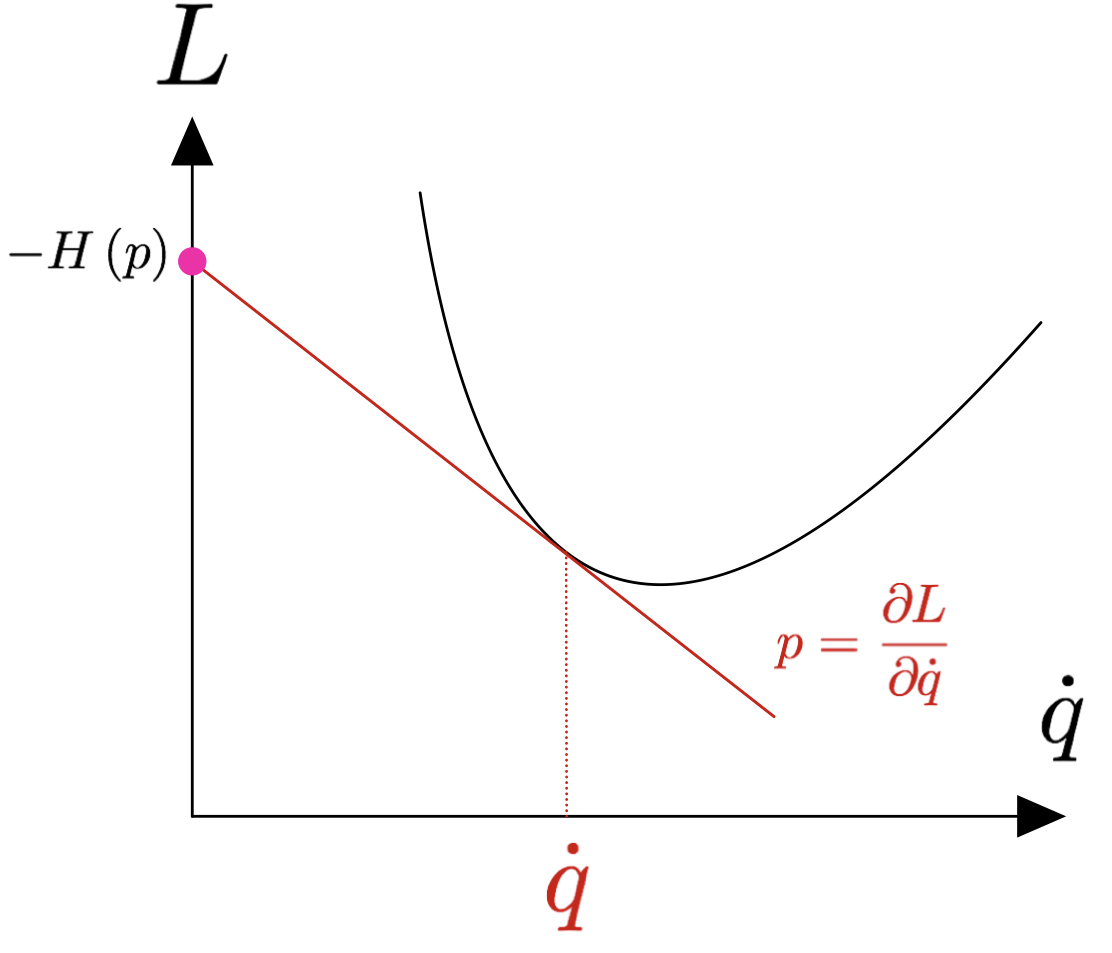
\includegraphics[width=0.5\textwidth]{grafico_lq.png}
    \caption{Gráfico de Lagrangiano v/s coordenada}
    \label{grafico_lq}
\end{figure}
La recta:$y+mx +n \implies L \qty(q,\dot{q}) - H(p,q) \implies H= p \dot{q}-L$

No es casualidad la forma de la Ecuación de Hamilton, ya que es como opera la transformada de Legendre.\\
Se debe mencionar que esta transformada se vera luego en termodinámica. Existen distintos potenciales termodinamicos y hay veces que se usa la energía interna en funcion de la entropia y el volumen o mediante la energia libre de gibbs en funcion de la temperatura y el volumen. la pregunta es son distintos, ya que mantienen el volumen en sus formulas y resulta que la energía de gibbs es una transformada de legendre.  $E= Q - TS$.
 \newpage
 
 \ss{Ejemplo: Oscilador ármonico}
 $$\mathcal{L} = \frac{1}{2}m \dot{q}^2 - \frac{1}{2}k q^2$$
 $$p = \pdv{\mathcal{L}}{\dot{q}}$$
 \en{\mathcal{H}= \frac{p^2}{2m} + \frac{1}{2} k q^2}
 Ecuaciones de Hamilton:\\
 $$\dot{q} = \pdv{\mathcal{H}}{p}$$
 $$\therefore \dot{q}= \frac{p}{m}$$
 $$\dot{p}= \pdv{\mathcal{H}}{q} $$
 $$\therefore \dot{p}=-kq$$
 
 
 Podemos derivar $\dot{q}$ y obtener que:
 \eq{\ddot{q}= \frac{\dot{p}}{m}}
Reemplazamos esta ecuación en la segunda ecuacion de hamilton y tenemos que 
\eq{\ddot{q}=-\frac{k}{m}q}
Con esto obtenemos las soluciones del oscilador armonico.\\
\sss{Trayectorias en espacio de fases}
En este caso, el hamiltoniano es constante.
 $$\mathcal{L} = \frac{1}{2}m \dot{q}^2 - \frac{1}{2}k q^2 =E$$
Se puede observar que en un grafico de p v/s q es una elipse centrada.
\begin{figure}[h!]
    \centering
    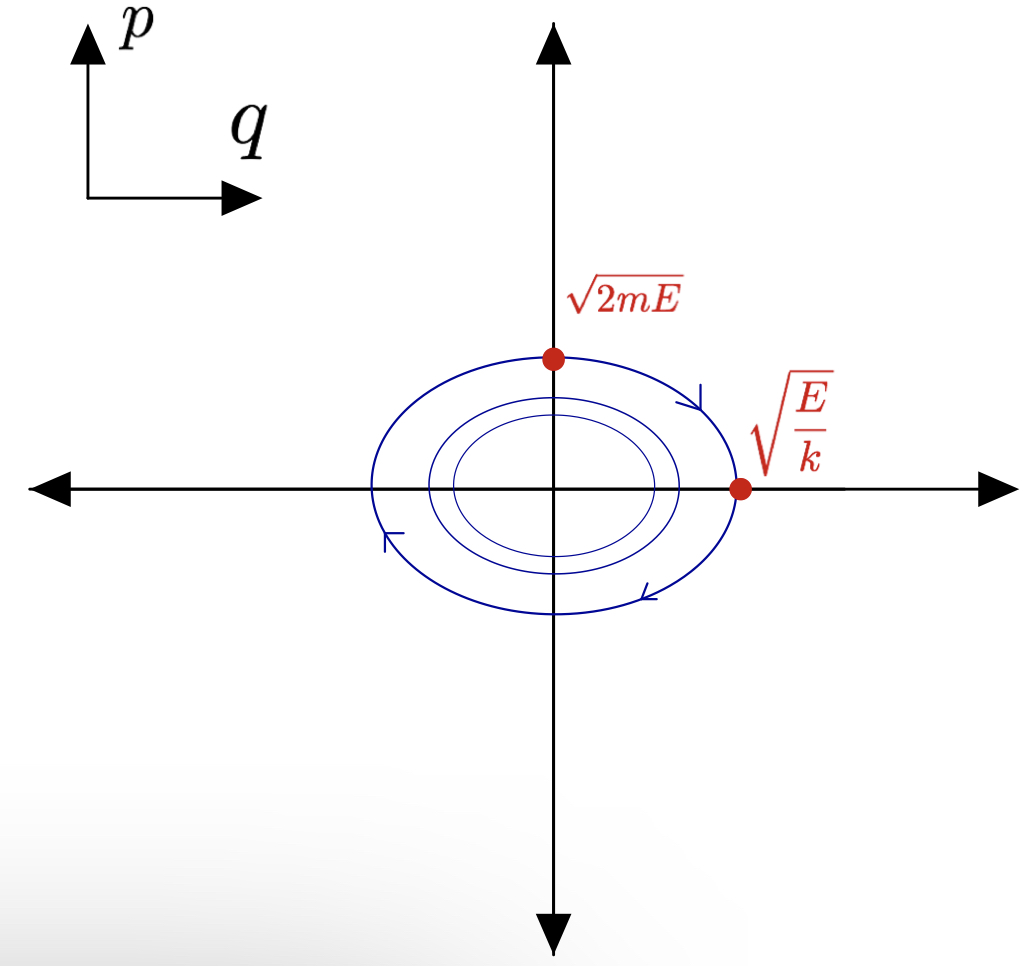
\includegraphics[width=0.35\textwidth]{grafico_pq.png}
    \caption{Gráfico de Lagrangiano v/s coordenada}
    \label{grafico_pq}
\end{figure}
Hay veces en el que las trayectorias se pueden intersectar y es en los puntos de equilibrio.\\
Una de las propiedades geometricas del espacio de fase. En la \fgref{grafico_pq} es el area de esto.\\
El area de la elipse obtenemos el periodo.
$$2\pi E \sqrt{\frac{m}{k}}= E \cdot T$$
Con esto se puede obtener el periodo del sistema mediante el área de la trayectoria.\\
Es interesante ver que si necesito saber el periodo este es \\
\eq{T= \dv{\textit{Area}}{E}}
Igualmente como $T=\frac{2 \pi}{\omega}$\\

\eq{\omega = \dv{E}{\frac{\texit{Area}}{2\pi}}}

Realizando un cambio de variable donde $J= \frac{1}{2 \pi} \texit{area}$\\
\eq{J= \frac{1}{2 \pi} \oint p \, d q}
\en{\omega = \dv{\mathcal{H}}{J}}
Esta J es llamada la variable de acción.
\sss{Pelota rebotando elásticamente con gravedad} 

La pelota desde una altura h el periodo en caer es 
\eq{t_{\texit{caida}}=\sqrt{\frac{2h}{g}}}
\eq{T=2 t_{\texit{caida}} = 2 \sqrt{\frac{2h}{g}}}
\en{\mathcal{H}= \frac{p^2}{2m} + mgq}
Ecuaciones de hamilton\\
\eq{\dot{q}= \pdv{\mathcal{H}}{p}= \frac{p}{m}}
\eq{\dot{p}= -\pdv{\mathcal{H}}{q}= mg}
\eq{\therefore \ddot{q}= -g}
Haremos estas trayectorias en el espacio de fases en \fgref{grafico_pq_pelota}.

\begin{figure}[h!]
    \centering
    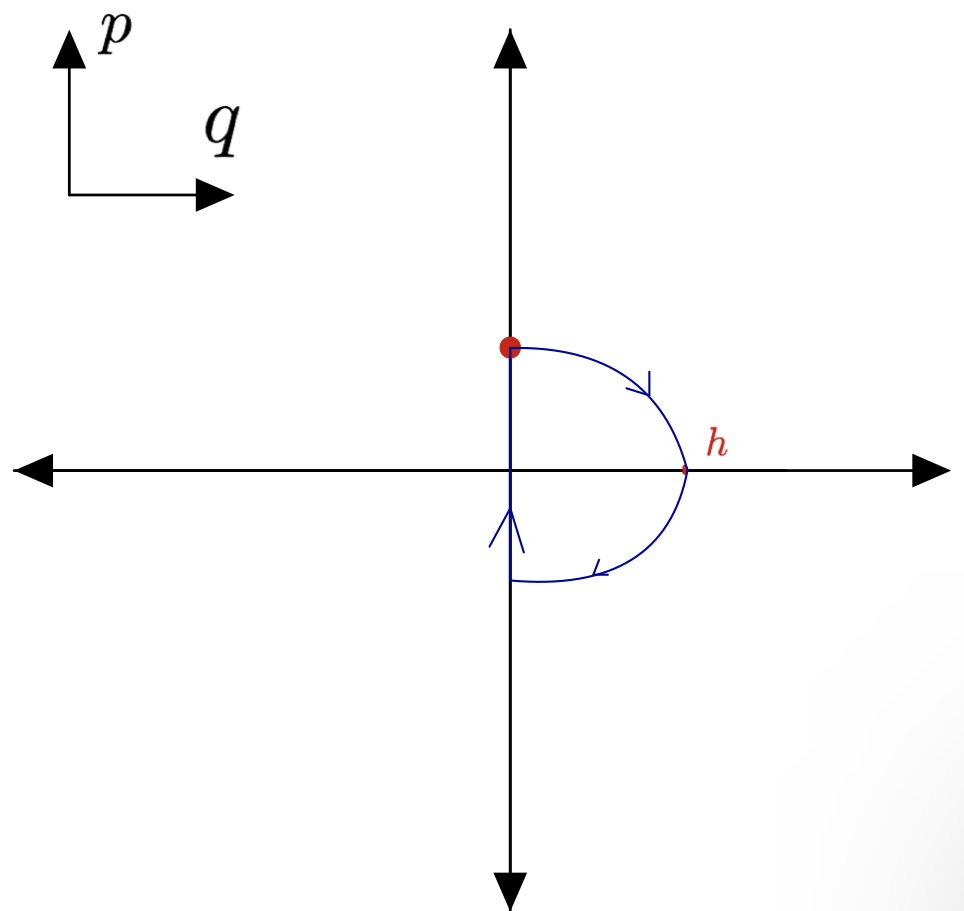
\includegraphics[width=0.35\textwidth]{espaciodefases_pq_pelota.png}
    \caption{Espacio de fases p v/s q pelota rebotando}
    \label{grafico_pq_pelota}
\end{figure}

\begin{align}
Area &=\oint p \, dq\\
&= 2 \int \limits_{0}^{\frac{E}{mg}} \sqrt{2m\qty(E-mgq)}dq\\
&=2 \frac{2}{-3mg} (2m(-E-mgq))\\
&=\frac{4}{3mg}\frac{\qty(2mE)^{\frac{3}{2}}}{2m}\\
&= \frac{4}{3} \frac{\sqrt{2m}}{mg}E^{\frac{3}{2}}
\end{align}

Si derivamos el area respecto a la energia tenemos
\begin{align}
\dv{A}{E}&= 2 	\frac{\sqrt{2m}}{mg}E^{\frac{1}{2}}\\
&= 2 \sqrt{\frac{2h}{g}}
\end{align}
\en{\dv{A}{E}=T \,\,\vline \,\, \dv{\mathcal{H}}{J}= \omega \,\, \vline \,\, J= \frac{\oint p \,dq}{2\pi} }
Area $=\oit p \, dq$ podemos derivar el area respecto a $\mathcal{H}$ y como esta no depende de q, puede entrar a la integral como una derivada parcial.
\begin{align}
	\dv{Area}{\mathcal{H}}&= \oint \pdv{p}{\mathcal{H}} \, dq\\
	&= \oint \frac{dq}{\pdv{\mathcal{H}}{p}}\bigg/ \pdv{\mathcal{H}}{p}= \dot{q}\\
	&=\oint \frac{q}{\dot{q}}\\
	&= \oint dt \\
	&= T\\
	&\therefore \dv{\mathcal{H}}{J}= \omega
\end{align}
 

\ss{Invariantes Adiabaticos}
$\mathcal{H}(q,p,\lambda(t))$, si el sistema es periodico si $\lambda=0$\\
Si $\lambda = \lambda(t)$ entonces el hamitoniano no se conserva.\\
Podemos calcular $\mathcal{H}(t)$?\\
\textit{Podemos si} $\Delta \lambda << \lambda$ sobre un periodo. Es decir, si el cambio transcurre lentamente, entonces el sistema se va a adaptando a este cambio y la variable de accion permanece constante. Se deformara el area de las trayectorias en el espacio de fases, pero \textbf{el area permanece constante}.\\
Un pendulo de longitud variable si es posible calcularlo. Y se puede notar que la amplitud aumenta cuando el largo es menor.
$$\frac{\theta_{max}`}{\theta_{max}}= \qty(\frac{l`}{l})^{3/4}$$


\end{document}